\chapter{Estado del Arte}\label{chapter:state-of-the-art}

% Argumentacion background

\section{Argumentación}

La argumentación es el proceso que consiste en producir elementos que justifiquen una afirmación. Una afirmación 
constituye una expresión de algo ocurrido, un juicio, una evaluación. Las premisas son los elementos que 
justifican o atacan las afirmaciones. Un argumento básico está dado por la relación entre una afirmación y una 
premisa, con dicha premisa estar atacando o apoyando la afirmación inicial. Un ejemplo básico constituye:

"\emph{Las vacunas previenen la diseminación de enfermedades}, por lo tanto \textbf{vacunarse es necesario}."

En el ejemplo se puede observar un argumento simple y algunas características propias de estos, la justificación 
(en \textbf{negro}) que apoya la afirmación (en \emph{itálico}), también se puede observar palabras conectoras 
que indican además de conexión, la dirección de esta.

Sobre esta han surgido diferentes marcos teóricos que buscan una metodología para su representación y estudio. 
Una de las más citadas constituye el Método o Modelo de Toulmin.

El Método Toulmin fue extrapolado del libro \emph{The Uses of Argument}[\cite{toulmin_2003}] escrito por Stephen E. Toulmin.
Este método divide los argumentos en seis partes: afirmación (claim), fundamento (grounds), 
justificación (warrant), calificador (qualifier), refutación (rebuttal) y respaldo (backing).
Mediante las afirmaciones se conoce el argumento principal que el autor quiere probar a la audiencia,
estas son respaldados con fundamentos siendo estos las evidencias y hechos en que se apoya el autor.
Las justificaciones pueden estar explícitas o implícitas y son suposiciones que vinculan los
fundamentos con las afirmaciones, estas a su vez pueden ser respaldadas por conocimiento.
El esquema introduce la posibilidad de otra sitaución válida a la establecida en las afirmaciones
mediante la refutación. Los calificadores son usados para dar más información de la calidad o seguridad
de las afirmaciones dadas. Un ejemplo de este esquema es:

\emph{[Se escucharon ladridos y aullidos en la distancia](fundamento), [probablemente](calificador) 
[haya perros en las cercanías](afirmación).}

En este ejemplo, además de las partes explícitas, se encuentran implícitas, la justificación 
(los perros son animales que ladran y aullan), el respaldo (se sabe que existen perros en la zona) y 
la refutación (Puede ser que hayan lobos o coyotes cerca). [\cite{toulminArgument}]
  
\section{Extracción de Argumentos}

El Procesamiento de Lenguaje Natural (\textbf{NLP} por sus siglas en inlgés \emph{Natural Language Processing}) es un 
subcampo de la Inteligencia Artificial (IA) que tiene como objetivo la comprensión del lenguaje humano por 
las computadoras. 
Mediante el uso de sus algoritmos es posible el procesamiento masivo de texto para la extracción de información 
relvante de este. Entre las tareas pertenecientes a dicho campo se encuentran Traducción Automática (Ref), 
Generación de Lenguaje Natural (Ref) y Extracción de Argumentos (EA).

\subsection{Estructuras Argumentativas}

Las estructuras argumentativas son las partes y sus relaciones de las cuales están compuestas la argumentación en los textos.
Estas se componen de dos elementos principales, las Unidades de Discurso Argumentativas (UDA) y los enlaces
existentes entre estas. Las UDA se definen como secciones consecutivas de texto que contienen carga argumentativa,
la definición de carga argumentativa es un poco difusa y varía en dependencia del método que se use para el análisis. 
Tanto los enlaces como las UDAs son clasificadas en dependencia de las etiquetas usadas, estas clasificaciones 
parten de los conceptos de premisa y afirmación para las UDA y ataque y apoyo para las relaciones. 

\subsection{Tareas de extracción de argumentos}

Dada las estructuras argumentativas en la EA se conciben las siguientes tareas pricnipales:

\begin{enumerate}
    \item Extracción de las UDA
    \item Clasificación de las UDA
    \item Extracción de las relaciones entre UDA
    \item Clasificación de las relaciones entre UDA
\end{enumerate}

Partiendo de esto se puede observar que las estructuras argumentativas de un texto constituyen un grafo dirigido 
en donde sus nodos representan las UDA y están anotados con el tipo de esta y sus vértices representan las 
relaciones entre las UDA y dichos vértices se anotan con el tipo de relación existente.

\begin{figure}[h!]
	\begin{center}
		\begin{center}
			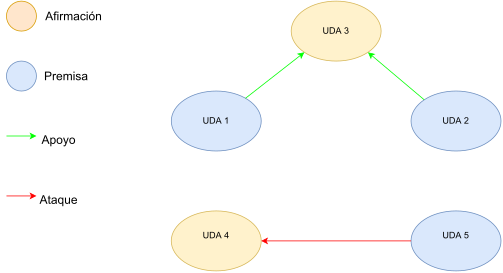
\includegraphics[scale=.3]{Graphics/Estructuras_argumentativas.png}
            % \includesvg[options]{Graphics/Estructuras argumentativas.svg}
        \end{center}
	    \caption{Estructuras Argumentativas}\label{fig:arg_struct}
	\end{center}
\end{figure}

\section{Preliminares de Extracci'on de Argumentos}

Varias investigaciones y propuestas han salido para dar respuesta a los problemas asociados a EA, mostrando
una variedad en enfoques y métodos.
En [\cite{palau2009argumentation}] se propone
el uso de modelos estadísticos como \emph{Naive Bayes} (\textbf{NB}) y \emph{Support Vector Machines} (\textbf{SVM}) 
para la clasificación de 
oraciones en argumentativas o no y en su rol argumentativo en caso de que sea argumentativa, en este
caso se asume que las componentes argumentativas son oraciones completas. Para la predicción de relaciones
se usa un enfoque basados en reglas con la creación de una Gramática Libre de Contexto. Las representaciones
de las oraciones se ven dadas por atributos elegidos a mano dado el conocimiento experto sobre la argumentación
en el tema tratado, elementos como adverbios, verbos, signos de puntuación, palabras clave, estadísticas del texto
(Tamaño de oración, distancia media de palabras) son usados para la extracción y clasificación de las UDA, además
se usan también como base en la creación de las relgas para la extracción de relaciones.

[\cite{goudas2015argument}] al igual que [\cite{palau2009argumentation}] clasifica las oraciones como
argumentativas o no mediante el uso de diferentes clasificadores como \emph{Naive Bayes}, \emph{Random Forest}, Regresión
Logística y \emph{Support Vector Machines}. En este trabajo se aumenta la grandularidad de la segmentación al permitir
la extracción de los segmentos que contienen la carga argumentativa de dentro de las oraciones previamente clasificadas
como tal, esto se realiza mediante la extracción de etiquetas BIO de las oraciones con el uso de un 
\emph{Conditional Random Field} (\textbf{CRF}). La predicción de las relaciones como un problema de clasificación
usando \emph{Support Vector Machine} para clasificar pares de UDA en relacionados o no. Atributos asignados a mano 
son usados en la extracción de UDA como posición de la oración en el texto, cantidad de verbos, comas, adverbios,
palabras, entidades en la oración, también se emplean gaceteras que guardan entidades relacionadas con el dominio 
especifico y palabras clave indicadoras de frases argumentativas. 

[\cite{stab2017parsing}] propone un mecanismo de segmentación basado en Conditional Random Fields. La clasificación
y predicción de relaciones es modelado conjuntamente como con dos clasificadores \emph{Support Vector Machine} y un problema
de Optimización Lineal Entero que encuentra la mejor estructura y asegurar una disposición arborea. En la segmentación
de las UDA se extraen por cada token su posición en el texto, si precede o sucede a un signo de puntuación, su parte de
la oración, la probabilidad de que sea el comienzo de una UDA dado sus tokens anteriores, entre otros. Para la extracción
y clasificación de relaciones se proponen otros conjuntos de atributos como la cantidad de sustantivos comunes entre
las componentes fuente y el objetivo, la presencia de indicadores argumentativos, representaciones vectoriales de tokens.

En [\cite{eger2017neural}] se enfocaron en
modelar el problema como un problema de etiquetado de secuencias, usando Redes Neuronales Recurrentes (\textbf{RNN}) como 
\emph{Long-Short Term Memory} (\textbf{LSTM}) en versiones bidireccionales capturando información desde ambos lados de la secuencia,
extrayendo información morfológica de las palabras mediante Redes Neuronales Convolucionales teniendo una capa final de
\emph{Conditional Random Field}. Realizaron experimentos al modelar el problema como uno de \emph{Dependency Parsing} cuyo problema
consiste en construir un árbol de dependencia que codifique las estructuras argumentativas. El problema fue modelado
como un problema de reconocimiento de entidades nombradas, en donde las entidades son las UDA.

[\cite{galassi2018argumentative}] propone el uso de redes residuales y en combinación con mecanismos de atención
para la creación de un modelo el cual, conjuntamente, clasifica el tipo de UDA y la relación existentes entre estas.
Este trabajo define el concepto de distancia argumentativa, añadiéndolo como feature y asume que las UDA ya fueron 
extraídas. En este caso además de la distancia argumentativa las secuencias son representadas por sus representaciones
vectoriales de GloVe.

En [\cite{dykes2020reconstructing}] se propone métodos basados en reglas para la extracción de argumentos sobre
textos en Twitter, estos métodos se centran en la confección de reglas basadas en anotaciones lingüísticas como
partes de la oración, lemas de palabras. La recuperación está basada en los esquemas argumentativos comunes presentes
en los textos. Este método apunta a una mayor precisión prescindiendo de recobrado. 

Se contempan disímiles enfoques al problema de EA desde una perspectiva enmarcada en modelos 
simbólicos, estadísticos y neuronales en versiones tanto secuenciales como end-to-end. 
Cada uno de estos modelos presentan sus ventajas y desventajas a la hora de contruirlos, 
extenderlos y comprender su funcionamiento. En modelos simbólicos se presenta una alta
precisión en dominios específicos debido a que estos se construyen teniendo en cuenta un
contexto dado. Estos modelos son poco escalables y difíciles de mantener ya que son construídos
a mano y dicho proceso requiere de conocimiento experto y tiempo. Modelos estadísticos son
característicos de usar conjuntos de atributos creados a mano, dichos atributos son difíciles
de encontrar, calcular y pueden no poseer relevancia en otros contextos diferentes a los que fueron creados. 
Además la necesidad de conocimiento experto es necesaria para su confección. Los modelos neuronales poseen
un mayor poder de adaptabilidad, en estos la entrada es codificada en una representación que es aprendida por
el mismo algoritmo, permitiendo seguir viable para distintos esquemas argumentativos. Los modelos simbólicos y 
estadísticos poseen la ventaja de poder explicar el porqué de los resultados devueltos cosa que se vuelve casi
imposible en modelos neuronales.

Dado que la EA es un proceso en el cual se necesita pasar por varias tareas, estas deben de ser completadas
de alguna forma. Una manera de completarlas es hacerla una a la vez, independiente una de otra y pasándole
la salida de etapas anteriores a las etapas siguientes. Esta manera secuencial de realizar las 
tareas es bastante simple y ayuda a la creación de modelos simples y con tareas definidas, aunque trae consigo 
la propagación de los errores a través del proceso y el no aprevechamiento de las interrelaciones entre variables 
computadas de procesos anteriores. Modelos \emph{end-to-end} en cambio poseen la habilidad de modelar el problema 
desde su inicio hasta su final de manera conjunta, mediante \emph{Multi-Task Learning} (\textbf{MTL}) se modelan
las tareas de manera conjunta creando modelos complejos aunque con una propagación de error menor.


% En los modelos propuestos existen algunos problemas relacionados con
% el uso independiente de modelos para el completamiento de la tareas asociadas a EA. Esto conlleva a la propagación
% de errores ya que las entradas de etapas posteriores presentan las errores de las etapas anteriores.
% También la no explotación de las interrelaciones entre variables debe ser tomado en cuenta, ya que se pierde
% información computada en etapas anteriores. Modelos end-to-end y 
% Multi-Task Learning han surgido para mitigar estos errores. En estos modelos el entrenamiento se hace de forma 
% conjunta y no secuencial, previendo la propagación de errores y también se aprenden las distintas tareas al mismo
% tiempo, pudiendo extraer las relaciones entre las diferentes tareas realizadas.
% La arbitrariedad y dificultad de extraer de los atributos creados a mano persiste en varios modelos [\cite{goudas2015argument}, \cite{palau2009argumentation}]
% además de que estos pueden ser difíciles de adaptar para otros documentos [\cite{eger2017neural}].
% La creación de modelos que usen representaciones aprendidas sin o poca intervención de conocimiento humano hace 
% que sean más robustos a los diferentes esquemas de argumentación pudiendo adaptarse a estos sin 
% realizarle cambios en este.

\section{Proyección de corpus}

La EA no es un campo de NLP que presenta una gran cantidad de datos anotados con los cuales se pueda realizar 
un entrenamiento, además de esto la gran mayoría de corpus existentes se encuentran en lenguajes como inglés o alemán,
haciendo difícil el desarrollo de esta rama en otros lenguajes.
La escasez de estos datos es en gran parte debida al elevado costo en dinero, tiempo y recursos humanos que se emplea
en su creación.

En orden de poder desarrollar la EA en otros lenguajes, como el español, se han investigado diferentes vertientes, 
proyección de etiquetas y transferencia directa. La proyección de etiquetas consiste en un algoritmo en donde se 
transfieren las etiquetas de un corpus anotado a nivel de tokens en un lenguaje origen hacia su traducción en un 
lenguaje objetivo. Transferencia directa se refiere a (TODO completar)
En [\cite{eger2018cross}] se muestra que la proyección constituye una mejor alternativa sobre la transferencia
directa y presentan un algoritmo para realizar la proyección de las etiquetas dadas las alineaciones de palabras.
El proceso se divide en varias partes.

\subsection{Traducción de oraciones}

La Traducción Automática consiste en el proceso de usar inteligencia artificial para
traducir texto de un lenguaje fuente a un lenguaje objetivo sin la intervención humana.
En la actualidad este campo ha dado un gran paso pasando de modelos estadísticos a modelos
neuronales llevando a tener traducciones de una alta calidad sin variar significativamente de la humana, 
condición necesaria para una buena proyección [\cite{eger2018cross}].

Por lo anterior es posible la traducción de corpus hacia otros lenguajes mediante las
herramientas existentes obteniendo una buena representación final, la cual se puede usar en la creación de
oraciones alineadas, primer paso para la proyección de etiquetas.

\subsection{Alineación de palabras}

La alineación de palabras consiste en encontrar las palabras generadas en el lenguaje objetivo por las 
palabras en el lenguaje fuente.
Este problema es atacado en los modelos IBM, modelos estadísticos de traducción automática que usan estos 
índices para obtener más información. Estos modelos son principalmente Bayesianos y han sido la base de
otras herramientas como FastAlign [\cite{dyer2013fastalign}] que incorpora una reducción sustancial del
tiempo de cómputo y además de una mejora al modelo, EFMARAL [\cite{ostling2016efficient}] que usa
Cadenas de Markov Monte Carlo. Modelos más recientes se han enfocado en explotar las representaciones
vectoriales de palabras y el uso de métodos de atención para la extracción de las
alineaciones [\cite{dou2021word}].

FOTO de EJEMPLO de ALINEACION

\subsection{Proyección de etiquetas}

La proyección de etiquetas consiste en transportar las etiquetas de las palabras en la secuencia origen
hacia las palabras de la secuencia destino tomando como datos las alineaciones entre estas. En [\cite{yarowsky2001inducing}]
se trata el problema de proyección de frases nominales, estas frases tienen como característica que son resistentes
a ser divididas en caso de ser traducidas, dicha propiedad se cumple para las UDA también, que aunque evidencian 
cambios en el orden de las palabras, mantienen la misma ventana. La proyección de UDA son más simples en el caso
que solamente se tiene en cuenta la ventana y las etiquetas en estas son constantes, no pasa con la proyección en
frases nominales las cuales pueden cambiar dentro de una ventana, por lo que algoritmos más simples existen
para esta tarea [\cite{eger2018cross}].

